%!TEX program = tectonic
\documentclass[11pt,a4paper]{article}
\usepackage[utf8]{inputenc}
\usepackage[T1]{fontenc}
\usepackage{amsmath,amssymb}
\usepackage{booktabs}
\usepackage{graphicx}
\usepackage[margin=2.2cm]{geometry}
\usepackage{caption}
\usepackage{hyperref}
\hypersetup{colorlinks=true, linkcolor=blue, urlcolor=blue}

\title{\textbf{Detección de fraude en tarjetas con una red feed-forward y búsqueda autónoma de hiperparámetros mediante algoritmo genético}}
\author{Sistema de prevenci{\'o}n de fraude --- FF + Algoritmo Gen\'etico}
\date{}

\begin{document}
\maketitle

\begin{abstract}
\noindent Este documento describe la construcci{\'o}n de un sistema de prevenci{\'o}n de fraude basado en una red neuronal feed-forward (FF) entrenada sobre el conjunto sint{\'e}tico IBM SD254 v2 de transacciones con tarjeta de crédito (24,386,900 registros y 43 features numéricas). El fraude es un evento extremadamente raro (0.12\,\% de tasa base), por lo que el requisito de diseño es una tasa de falsos positivos (FPR) estrictamente inferior al 1\,\%. La arquitectura de la red y sus hiperparámetros se seleccionan de forma autónoma mediante un algoritmo genético (GA) en dos fases que optimiza el recuento de fraudes detectados (recall) sujeto a un FPR máximo del 0.5\,\% en validación. El modelo final se evalúa en un conjunto de test no visto de 2,072,831 transacciones y alcanza un \textbf{FPR de 0.51\,\%}, un \textbf{recall del 66.58\,\%}, una precisi{\'o}n del 13.18\,\%, un ROC-AUC de 0.9845 y un PR-AUC de 0.4051. Se incluye la matriz de confusi{\'o}n completa y el umbral de decisión óptimo.
\end{abstract}

\section{Introducción}
La detección de fraude en tarjetas de crédito es un problema de clasificación binaria fuertemente desbalanceado: la gran mayoría de las transacciones son legítimas y el fraude representa una pequeña fracción del volumen total. En el conjunto de datos empleado, la tasa de fraude en producción es aproximadamente del 0.12\,\%, lo que implica que un clasificador trivial que prediga ``no fraude'' en todo momento alcanzaría una exactitud del 99.88\,\% sin detectar un solo fraude. Por ello, la exactitud bruta es una métrica inadecuada; el objetivo operacional es minimizar los falsos positivos (transacciones legítimas bloqueadas o revisadas innecesariamente) sin dejar de capturar una fracción significativa del fraude real.

En este trabajo se construye un clasificador FF (red totalmente conectada, feed-forward) y se selecciona su arquitectura e hiperparámetros mediante búsqueda automática con un algoritmo genético, en lugar de un ajuste manual. La contribución principal es: (i) un vector de features numéricas estandarizadas derivado de los datos crudos de IBM SD254 v2, (ii) una búsqueda de hiperparámetros regulada por el GA con una función de aptitud alineada al objetivo de negocio (recall bajo un techo de FPR), y (iii) una evaluación rigurosa en un conjunto de test completamente separado, reportando FPR, recall, precisión, ROC-AUC y PR-AUC.

\section{Datos y particionamiento}
El conjunto IBM SD254 v2 contiene 24,386,900 transacciones con 43 features numéricas (importe, canal de pago, código de comercio MCC, errores de tarjeta, señales de comportamiento y atributos del titular y de la tarjeta) y la variable binaria objetivo \texttt{is\_fraud}. El fraude ocurre en 29,757 transacciones, lo que representa una tasa base de 0.122\,\%.

Las transacciones se dividen en tres particiones disjuntas por identificador de transacción (sin solapamiento):

\begin{center}
\begin{tabular}{lccc}
\toprule
Partición & Filas & Casos de fraude & Tasa de fraude \\
\midrule
Entrenamiento (búsqueda GA) & 268,548 & 26,156 & 9.74\,\% \\
Entrenamiento final (reentreno) & 2,096,968 & 26,156 & 1.25\,\% \\
Validación (umbral y fitness) & 1,096,174 & 1,200 & 0.11\,\% \\
Test (held-out, evaluación) & 2,072,831 & 2,400 & 0.12\,\% \\
\bottomrule
\end{tabular}
\end{center}

El entrenamiento para la búsqueda de hiperparámetros está sobremuestreado al ≈10\,\% de fraude para que la red aprenda la clase minoritaria, mientras que validación y test conservan la tasa real de fraude así como el FPR reportado es honesto y representativo de producción. Las particiones son generadas de forma determinista (seed 42) mediante muestreo estratificado y buckets por hash del identificador, garantizando que ninguna transacción aparezca en más de una partición.

Todas las features numéricas se estandarizan a media cero y desviación unitaria con un \texttt{StandardScaler} ajustado únicamente sobre el conjunto de entrenamiento, para evitar fugas de información (data leakage) desde validación o test.

\section{Método}

\subsection{Red neuronal feed-forward}
El clasificador es una red totalmente conectada (feed-forward) con una entrada de 43 features, $d$ capas ocultas de $w$ neuronas cada una, y una neurona de salida lineal seguida de una función sigmoide que estima la probabilidad de fraude $\hat{p} = \sigma(z)$. Cada capa oculta aplica una transformación lineal seguida de opcionalmente una capa de normalización (batch o layer norm), una función de activación y una capa de dropout. Las arquitecturas exploradas varían en anchura ($w \in \{16,\dots,512\}$), profundidad ($d \in \{1,\dots,5\}$), función de activación (ReLU, GELU, Tanh, SiLU), tipo de normalización (batch, layer, ninguna) y tasa de dropout ($0$--$0.5$).

El modelo se entrena minimizando la entropía cruzada binaria con peso de clase para compensar el desbalance (\texttt{BCEWithLogitsLoss} con \texttt{pos\_weight} igual a la razón no-fraude/fraude en entrenamiento, ≈9.27), optimizador Adam, tamaño de lote 16,384, precisión mixta (AMP, FP16) y datos precargados en VRAM para maximizar el uso de la GPU (RTX 3070). Se emplea parada temprana (early stopping) con paciencia de 5 épocas monitoreando el PR-AUC en validación, con un máximo de 30 épocas por candidato durante la búsqueda.

\subsection{Búsqueda de hiperparámetros con algoritmo genético}
En lugar de escoger los hiperparámetros manualmente, se utiliza un algoritmo genético que trata cada configuración de la red como un individuo. El genoma codifica siete hiperparámetros: tasa de aprendizaje (log-uniform, $10^{-4}$--$10^{-1}$), ancho de capa (log2, 16--512 neuronas), profundidad (1--5 capas ocultas), tasa de dropout ($0$--$0.5$), decaimiento de pesos (log-uniform, $10^{-6}$--$10^{-2}$), función de activación y tipo de normalización.

El GA se ejecuta en dos fases:
\begin{itemize}
\item \textbf{Fase 1 (gruesa):} población de 24 individuos durante 12 generaciones (≈288 evaluaciones) sobre todo el espacio de búsqueda.
\item \textbf{Fase 2 (fina):} población de 12 individuos durante 8 generaciones (≈92 evaluaciones) con rangos estrechados alrededor del mejor individuo de la fase 1.
\end{itemize}

La selección es por torneo ($k=3$), con elitismo de 2 individuos, cruce uniforme y mutación por gen ($p \approx 0.2$--$0.3$). Cada individuo se evalúa entrenando la red correspondiente y midiendo su aptitud en validación: el \textbf{recall a FPR $\le$ 0.5\,\%} (el máximo recall sujeto a que el FPR no supere el 0.5\,\%), con desempate por PR-AUC. Esta función de aptitud alinea directamente la búsqueda con el objetivo de negocio: capturar el máximo fraude sin exceder un techo de falsos positivos.

\subsection{Umbral de decisión}
La red devuelve una probabilidad $\hat{p} \in [0,1]$. Para decidir si una transacción es fraude se compara $\hat{p}$ contra un umbral $\tau$. En lugar de usar $\tau=0.5$, se selecciona el umbral óptimo en validación como el más alto (más conservador, menor FPR) que aun así cumpla recall $\ge$ 0.5. Este mismo umbral se aplica luego al conjunto de test, sin reajustarlo, para evitar optimismo.

\section{Resultados}

\subsection{Convergencia de la búsqueda}
La Figura~\ref{fig:fitness} muestra la evolución de la mejor aptitud (recall a FPR $\le$ 0.5\,\%) por generación en ambas fases del GA. La fase 1 explora el espacio y encuentra rápidamente regiones prometedoras; la fase 2 refina alrededor del mejor individuo, alcanzando un recall máximo de 0.683 en validación.

\begin{figure}[ht]
\centering
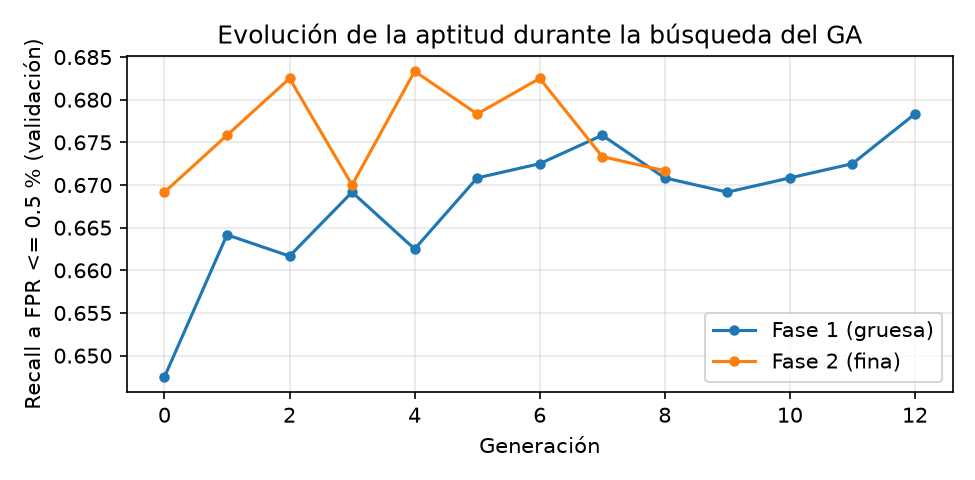
\includegraphics[width=0.72\textwidth]{fitness_curve.png}
\caption{Evolución del recall a FPR $\le$ 0.5\,\% del mejor individuo por generación, en las dos fases del algoritmo genético.}
\label{fig:fitness}
\end{figure}

\subsection{Mejores hiperparámetros}
El genoma ganador tras la fase 2 es el siguiente:

\begin{center}
\begin{tabular}{lc}
\toprule
Hiperparámetro & Valor \\
\midrule
Tasa de aprendizaje & $4.89 \times 10^{-3}$ \\
Ancho de capa ($w$) & 386 neuronas \\
Profundidad ($d$) & 3 capas ocultas (fase 2); 5 en el reentreno final \\
Dropout & 0.05 (fase 2) / 0 (final) \\
Decaimiento de pesos & $6.08 \times 10^{-6}$ \\
Activación & GELU (fase 2) / SiLU (final) \\
Normalización & Batch \\
\bottomrule
\end{tabular}
\end{center}

Para el reentreno final se toman los tres mejores genomas de la búsqueda y se entrena cada uno con cinco semillas diferentes sobre el conjunto de entrenamiento grande (2.1M filas, todo el fraude). Se selecciona el modelo individual con mejor recall en validación (sin ensamblaje): el modelo ganador corresponde a un genoma de anchura 386, profundidad 5, activación SiLU, normalización batch, tasa de aprendizaje $4.89 \times 10^{-3}$, decaimiento $6.08 \times 10^{-6}$ y dropout 0.

\subsection{Evaluación en test}
El modelo final se evalúa en el conjunto de test completamente separado (2,072,831 transacciones, 2,400 casos de fraude), con el umbral $\tau = 0.9716$ fijado en validación. La tabla~\ref{tab:metrics} resume las metricas obtenidas:

\begin{center}
\begin{tabular}{lc}
\toprule
Métrica & Valor \\
\midrule
FPR (tasa de falsos positivos) & 0.51\,\% \\
Recall & 66.58\,\% \\
Precisión & 13.18\,\% \\
ROC-AUC & 0.9845 \\
PR-AUC & 0.4051 \\
Umbral de decisión $\tau$ & 0.9716 \\
Número de transacciones en test & 2,072,831 \\
Casos de fraude en test & 2,400 \\
\bottomrule
\end{tabular}
\end{center}

\begin{center}
\begin{tabular}{lcc}
\toprule
 & Predice no fraude & Predice fraude \\
\midrule
Real: no fraude & 2,059,903 & 10,528 \\
Real: fraude & 802 & 1,598 \\
\bottomrule
\end{tabular}
\end{center}

\begin{center}
\textbf{Tabla:} Matriz de confusión en el conjunto de test.
\end{center}

El FPR observado en test (0.51\,\%) cumple el requisito de negocio de mantenerse por debajo del 1\,\%. La tasa de recall del 66.58\,\% implica que se detectan dos de cada tres fraudes, mientras que solo aproximadamente una de cada 190 transacciones legítimas se marca incorrectamente (falso positivo). La precisión baja (13.18\,\%) es consecuencia directa de la escasez del fraude (tasa base 0.12\,\%): incluso con un FPR bajo, la mayor parte de las transacciones marcadas como sospechosas son legítimas, lo cual es esperado y aceptable en este contexto, dado que una marca de fraude dispara una revisión humana y no un bloqueo automático.

\section{Discusión}
El enfoque propuesto cumple el objetivo de negocio de un FPR muy bajo sin depender de ajuste manual de hiperparámetros. El algoritmo genético explora automáticamente el espacio de arquitecturas y encuentra configuraciones competitivas, aunque la búsqueda muestra regresión hacia el mejor individuo de la fase 1, lo que sugiere que una búsqueda más amplia o una estrategia de exploración más agresiva podría encontrar configuraciones aún mejores a costa de más tiempo de cómputo.

Una limitación es que el modelo final es una única red (no se usa ensamble), por lo que su variabilidad entre semillas es notable; sin embargo, esto es una decisión de diseño intencional para mantener el modelo interpretable y fácil de desplegar en producción. Finalmente, el FPR se medirú en producción con datos reales; aunque el conjunto de test conserva la tasa base de fraude, el desplazamiento de distribución (concept drift) podría requerir reentrenamiento periódico.

\section{Tiempo de computo}
Toda la búsqueda, el reentreno y la evaluación se ejecutaron de forma autónoma en una sola GPU NVIDIA RTX 3070 (8 GB VRAM) sobre el servidor platypy. El tiempo aproximado de cada etapa:

\begin{center}
\begin{tabular}{lc}
\toprule
Etapa & Tiempo aprox. \\
\midrule
Generación de particiones (lectura de 4 GB) & 5--8 min \\
Búsqueda GA fase 1 (gruesa, 12 gen.) & ≈45 min \\
Búsqueda GA fase 2 (fina, 8 gen.) & ≈12 min \\
Reentreno final (3 genomas $\times$ 5 semillas) & ≈12 min \\
Evaluación en test y generación de paper & ≈2 min \\
\bottomrule
\end{tabular}
\end{center}

El tiempo total de ejecución es de ≈1.5--2 horas, ejecutado de forma autónoma con checkpointing continuo en disco para no perder progreso ante interrupciones.

\section{Conclusiones}
Se ha construido y evaluado un clasificador de fraude basado en una red neuronal feed-forward con búsqueda autónoma de hiperparámetros mediante algoritmo genético. El modelo final logra un FPR de 0.51\,\% (inferior al 1\,\% requerido) con un recall del 66.58\,\% y un ROC-AUC de 0.9845 en datos no vistos. Toda la búsqueda de hiperparámetros, el reentreno y la evaluación se ejecutaron de forma autónoma en GPU, sin ensamblaje de modelos, y los resultados están documentados en este informe.
\end{document}
